\documentclass[margin = 10pt]{standalone}
\usepackage{xcolor}
\usepackage{tikz}
\usepackage{pgfplots}
\pgfplotsset{
compat = 1.18
}

\begin{document}
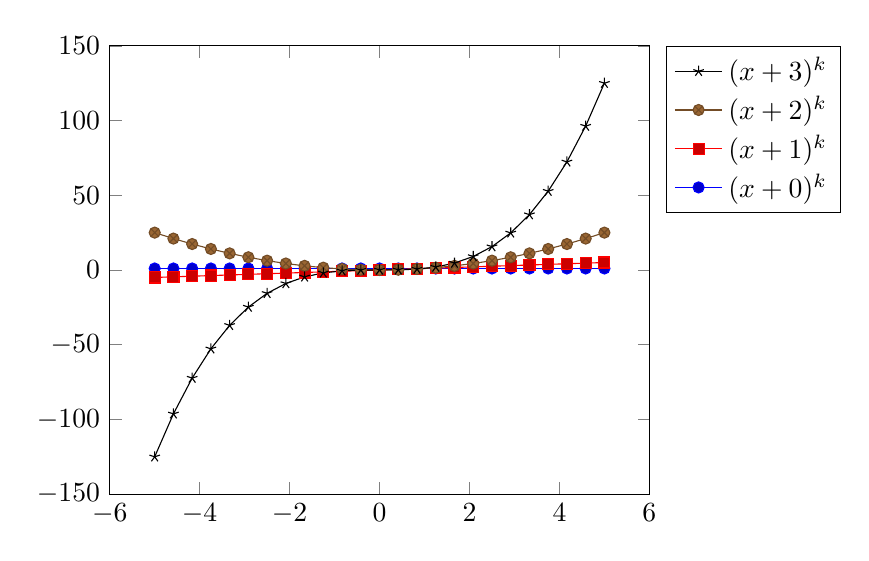
\begin{tikzpicture}[remember picture]
\begin{axis}[
    % 图例的设置        
    legend style = {
    	% 设置图例文字对齐方式
    	legend cell align = left,
    	%设置图例水平显示的例数量
    	legend columns = 1,
        % 设置图例中 小图的对齐位置
    	cells = {anchor= east},
    	% 设置图例锚点
    	anchor = north east,
    	% 图例的位置
        % at = {($(current bounding box.north west) - (0mm, 0mm)$) },
    	% 设置图例位置 
    	legend pos= outer north east,
    	legend entries={
    	    $(x+0)^k$,
    	    $(x+1)^k$,
    	    $(x+2)^k$,
    	    $(x+3)^k$},
        },
    reverse legend,
    ]
    
    
\addplot {x^0};
\addplot {x^1};
\addplot {x^2};
\addplot {x^3};
% \addlegendentry{A1}
\end{axis}
\end{tikzpicture}
\end{document}